\documentclass[spanish]{beamer}
\usetheme{Copenhagen}
\usepackage[utf8]{inputenc}
\usepackage[spanish]{babel}
\usepackage{graphicx}

\title{Unidad Aritmética Lógica}
\author{Gonzalo Vaca}

\begin{document}
\maketitle

\begin{frame}
    \frametitle{ALU}
    \centering
    
\includegraphics[width=0.8\textwidth]{img/alu_example.png}
\end{frame}

\begin{frame}
    \frametitle{RTL: Register Transfer Level}
    \centering
    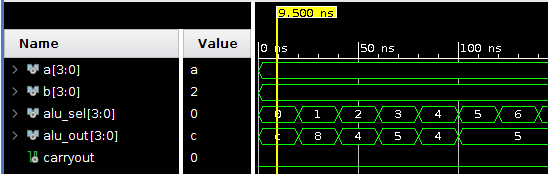
\includegraphics[width=\textwidth]{img/rtl_sim.png}
\end{frame}

\begin{frame}
    \frametitle{RTL: Register Transfer Level}
    \centering
    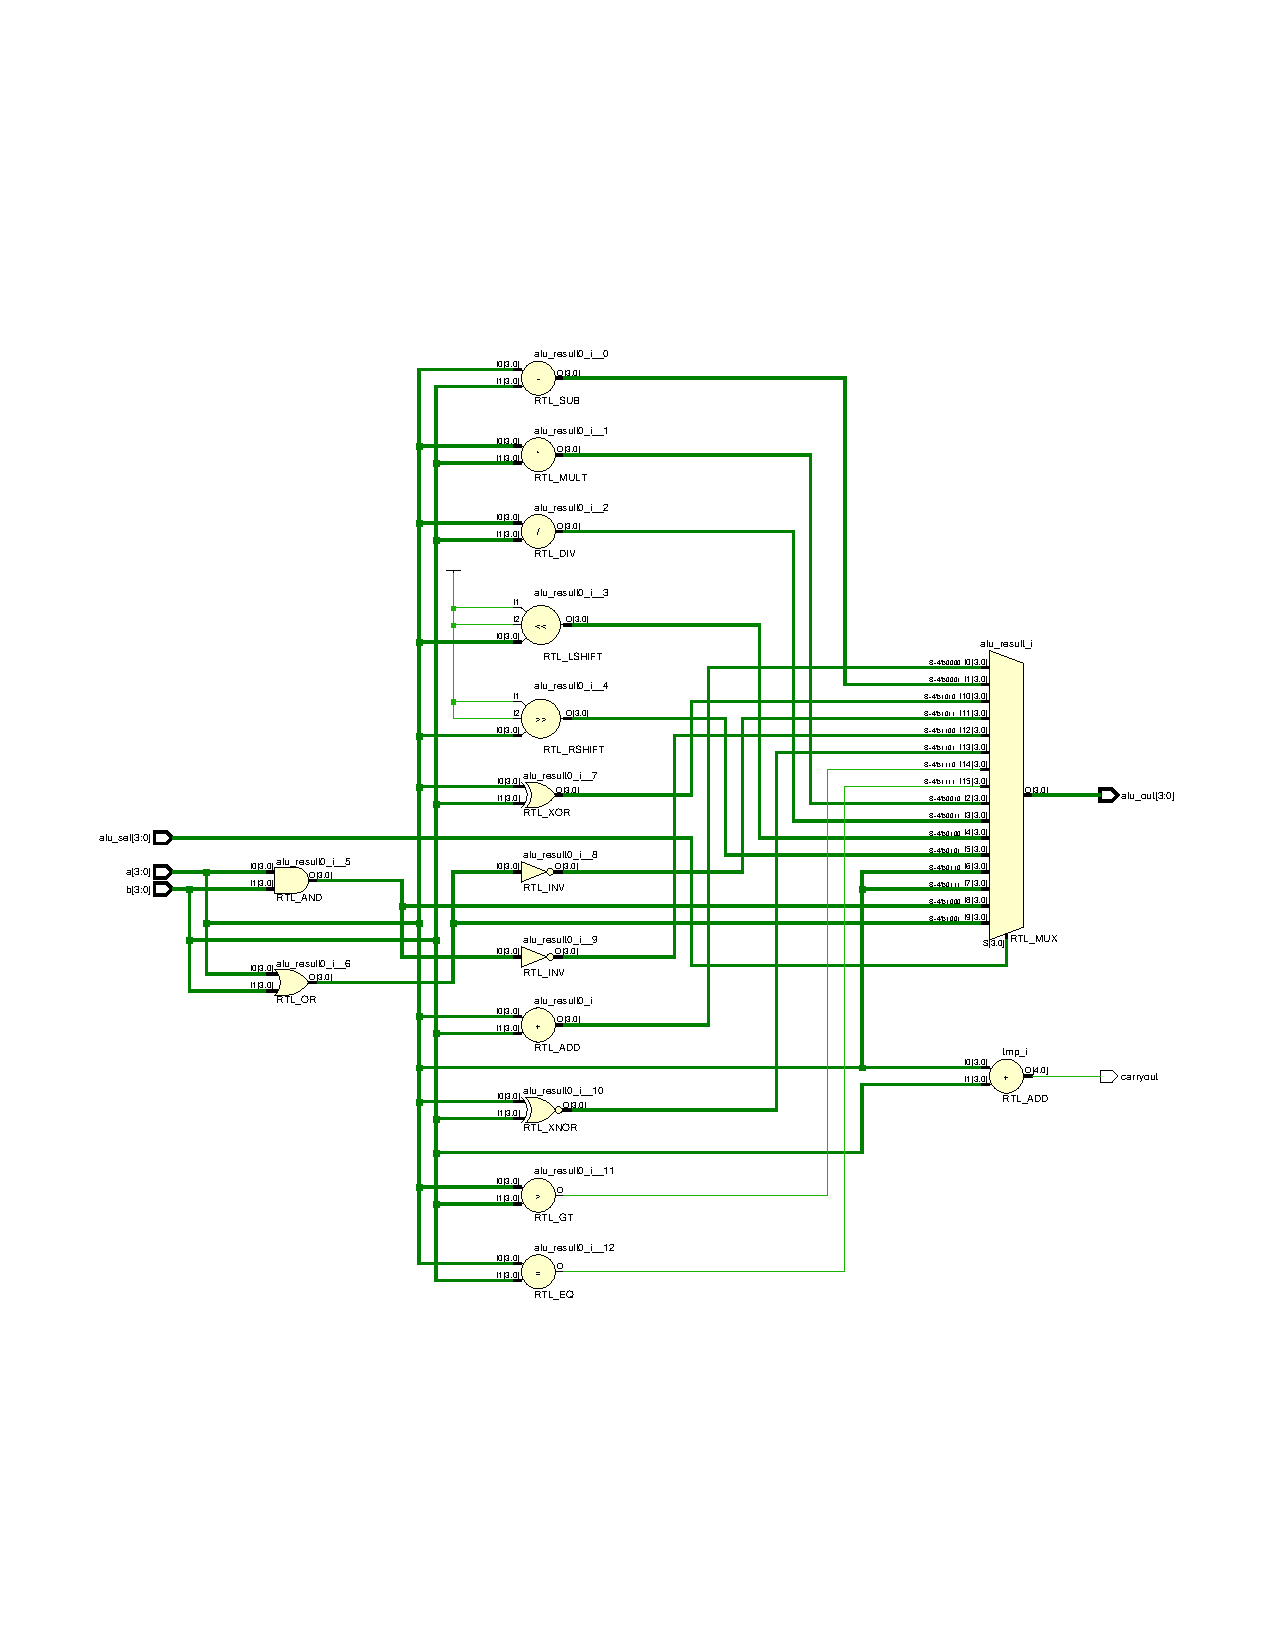
\includegraphics[height=10cm]{img/rtl_schematic.pdf}
\end{frame}

\begin{frame}
    \frametitle{Síntesis}
    \centering
    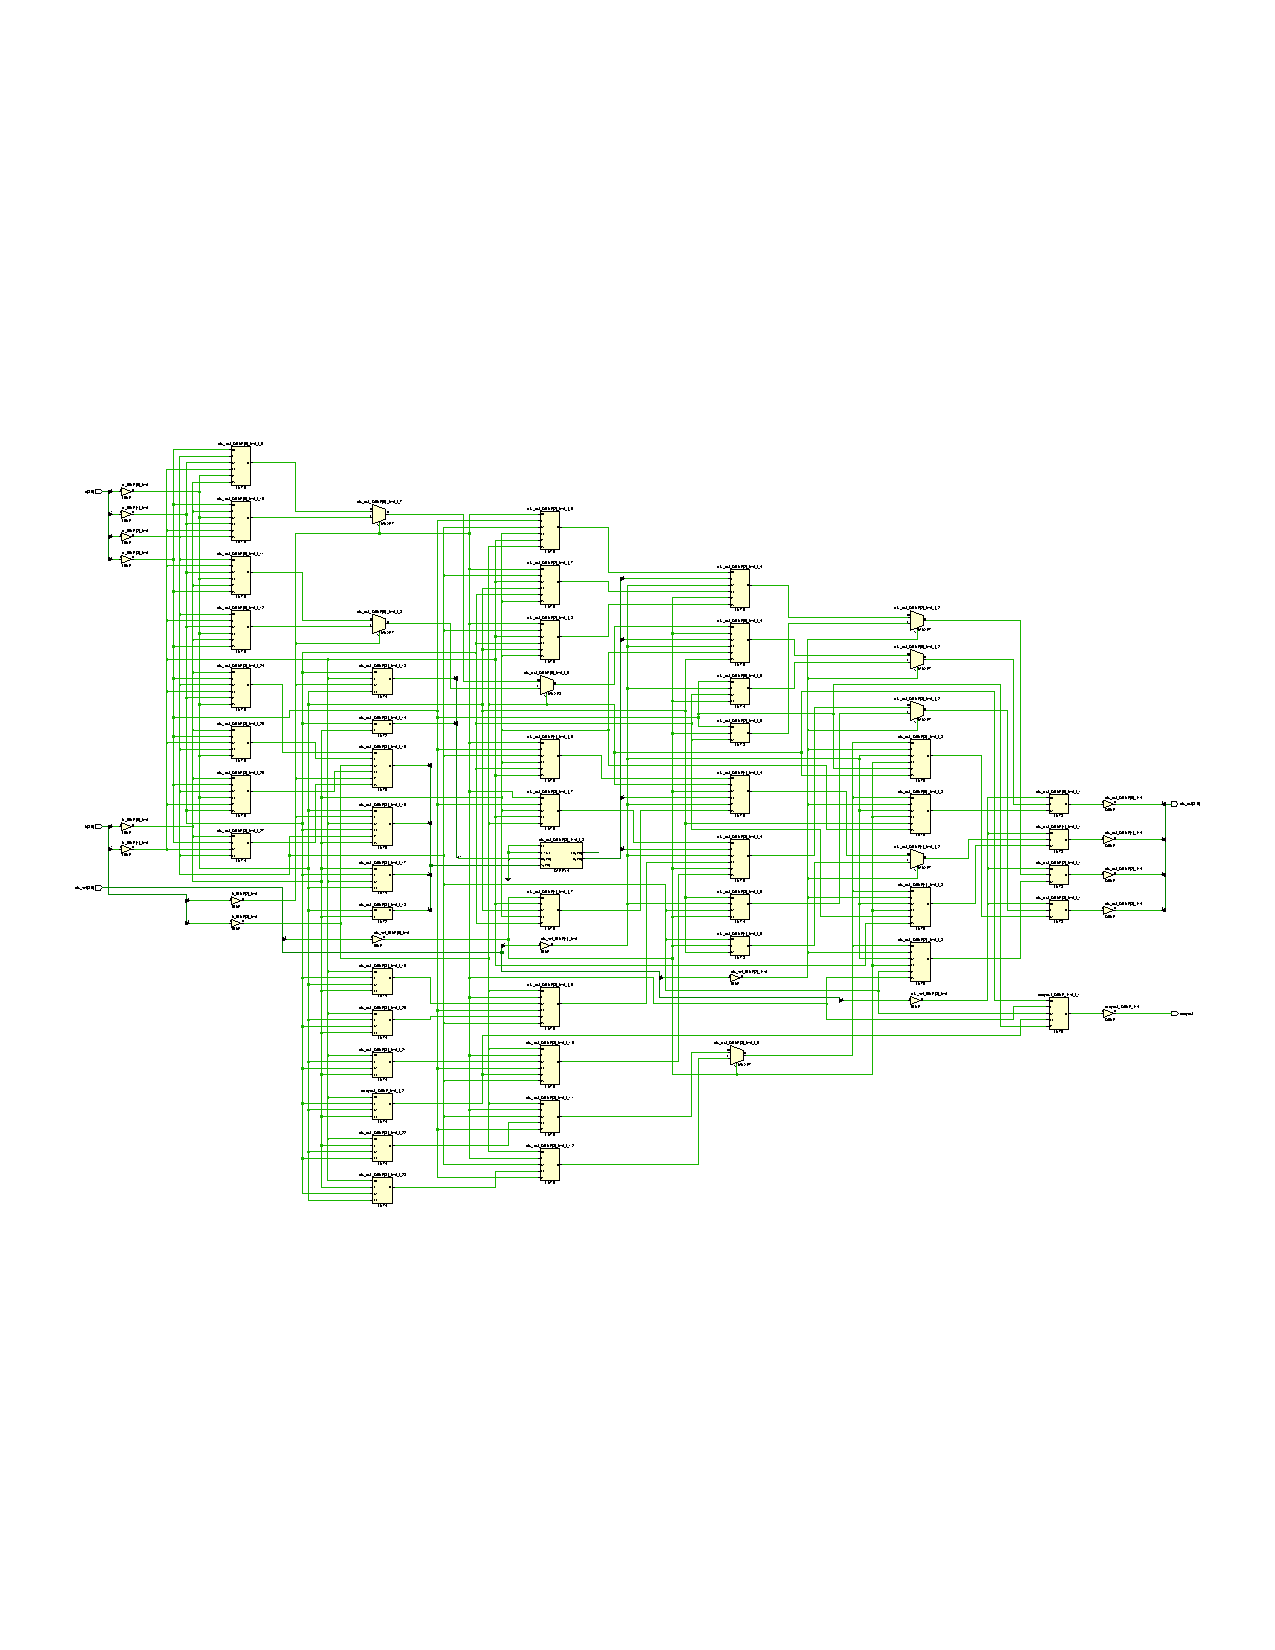
\includegraphics[height=10cm]{img/syn_schematic.pdf}
\end{frame}

\begin{frame}
    \frametitle{Implementación}
    \centering
    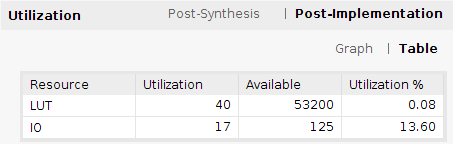
\includegraphics[width=0.8\textwidth]{img/imp_table.png}
\end{frame}

\begin{frame}
    \frametitle{Implementación}
    \centering
    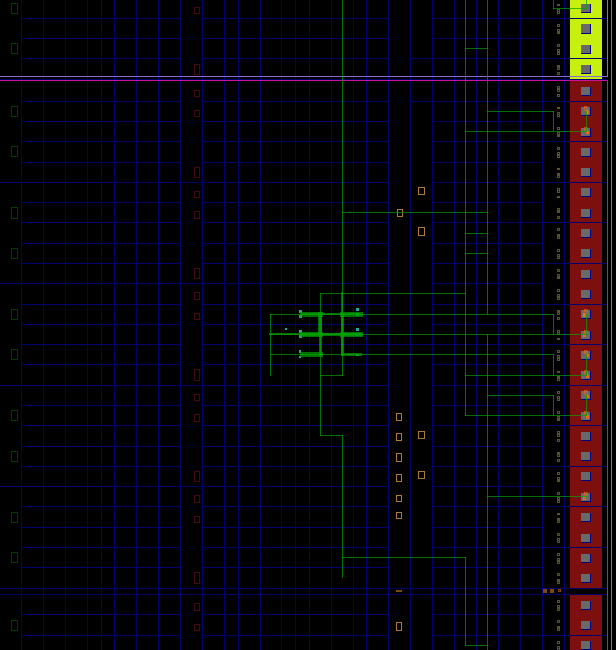
\includegraphics[width=\textwidth]{img/imp_device.png}
\end{frame}

\begin{frame}
    \frametitle{Montaje}
    \centering
    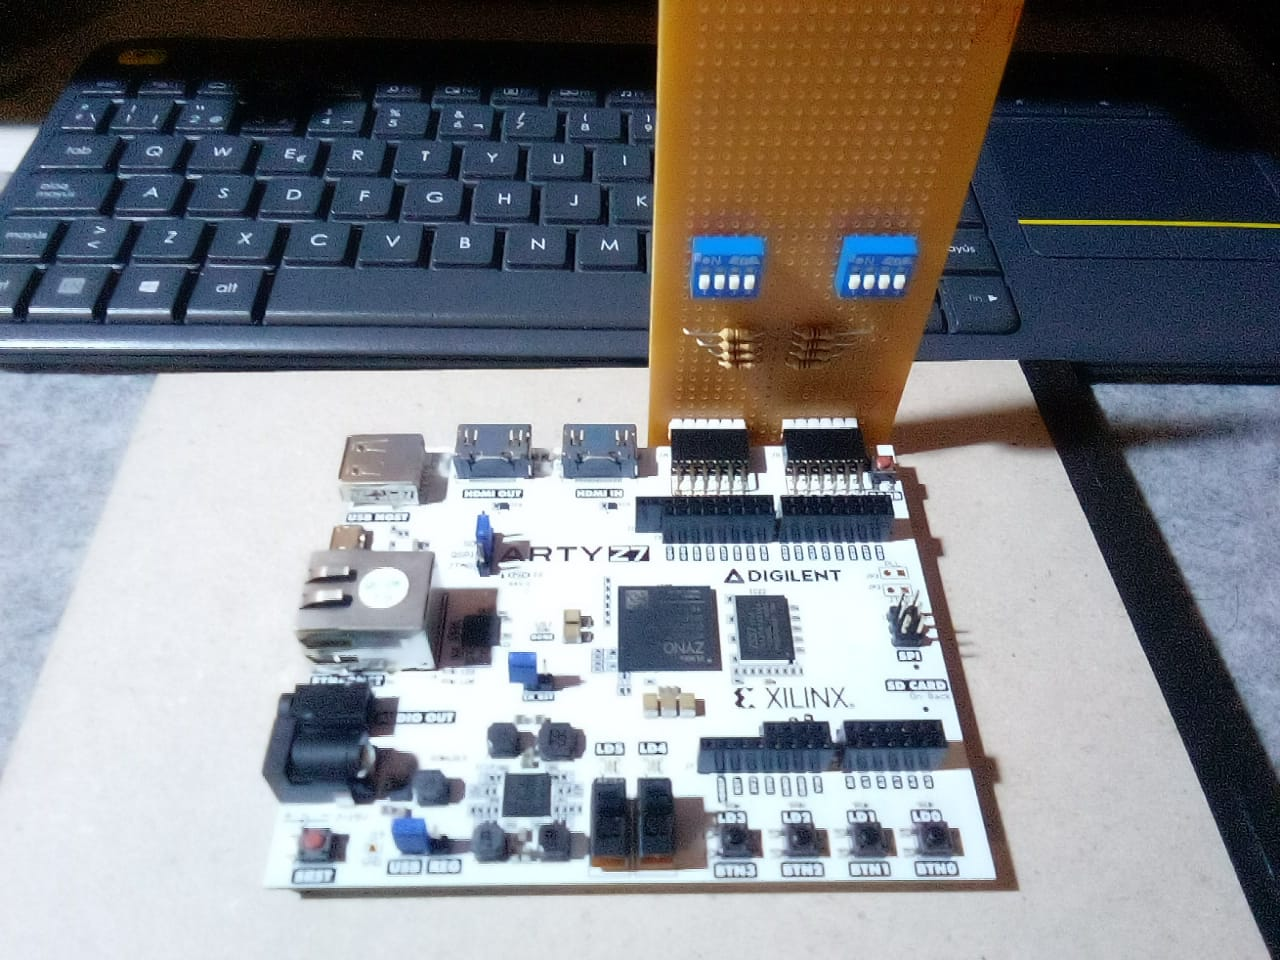
\includegraphics[width=\textwidth]{img/montaje.jpeg}
\end{frame}

\end{document}
